\documentclass[a4paper]{report}
\usepackage{a4}
\usepackage{doku}
\usepackage[ngerman]{babel}
\usepackage{longtable}
%\usepackage[draft]{graphicx}
\usepackage{nofloat}
\usepackage{graphicx}
\usepackage{tikz}
%\usepackage{graphics}
\usepackage{color}
\usepackage[dvips]{epsfig}
\usepackage{bbm}
\usepackage[utf8]{inputenc}
\usepackage{nomencl}
\usepackage[normalem]{ulem}
\usepackage[]{listings}

\newcommand{\ve}[1]{\mbox{\boldmath$#1$}}
\newcommand{\ma}[1]{\mbox{\boldmath$#1$}}
\newcommand{\eR}{\mbox{$\varepsilon I\;R$}}
\renewcommand{\today}{10.Dezember 2011}
\lstset{language=C++,tabsize=2,breaklines=true,breakatwhitespace=true, numbers=left}

\begin{document}

\begin{titlepage}
        \setcounter{page}{1}
        \let\footnotesize\small
        \let\footnoterule\relax
        \headsep 1.5cm
        \vskip -4cm
        \centerline{\Huge\bf Technische Universit\"at Braunschweig}
        \vskip 3.4cm
        \begin{center}
            \begin{minipage}[t][7cm][c]{13.5cm}
                \begin{center}
                    {\large{Teamprojekt}\par}
                    \vskip 0.5cm
		    {\LARGE\bf Koodinierte Ballsuche mit }
                    \vskip 0.25cm
                    {\LARGE\bf mobilen Robotern}
                    \vskip 0.5cm
                    {\Large\bf Martin Mikolas, Markus Reschke, Johannes
		    Starosta}
                    \vskip 0.25cm


                    {\large\bf Betreuer:
                    \begin{tabular}[t]{c}{René Iser}\end{tabular}}
                    \vskip 0.75cm
                    {\large\bf{\today}\par}
                \end{center}
            \end{minipage}
        \end{center}
        \vskip 1.5cm
        \begin{figure}[h]
            \begin{center}
							
\includegraphics{TU-Logo}
            \end{center}
        \end{figure}



        \vskip 1cm
        \centerline{\LARGE\bf Institut f\"ur Robotik und Prozessinformatik}
            \vskip 1cm
        \centerline{\LARGE\bf Prof.~Dr.~F.~Wahl}




    \end{titlepage}

    \declaration{den \today}

    \setcounter{footnote}{0}
    \pagenumbering{roman}
    \begin{abstract}Bei der vorliegenden Ausarbeitung handelt es sich
      um die Dokumentation unseres Teamprojektes zur ,,Koordinierten
      Suche mit mobilen Robotern''. Wir werden zunächst die
      Vorarbeiten vorstellen, auf denen wir ausbauten, bevor wir unser
      System näher vorstellen. Zum Schluss folgt noch eine kritische
      Bewertung unserer Ergebnisse.
    \end{abstract}

%    \raisebox{-12cm}{\hspace{5cm}\huge \textsc{To Loriot}}
 %   \newpage

%    \markright{Danksagungen}
%    \quote{ { \bf \Large  Danksagungen } \originalTeX
%    \\
%    \\
%    Unser Teamprojekt wäre nicht möglich gewesen, wenn wir nicht auf
%    wesentliche Vorarbeiten hätten zirück
%    I am very grateful to many people who helped me during my thesis in various
%    manners.
%    First, I wish to thank the entire staff of the Institute for Robotics and
%    Process Control for their helpful discussions and the truly great working atmosphere.
%    Particularly, I would like to thank Erich Kozlowski for his
%    helpful advice and tremendous encouragement during my student jobs at the Institute
%    and especially throughout this work.
%    Moreover, I am indebted to my family and my friends for their overwhelming
%    support throughout the last years.
%    Furthermore, I wish to thank Hans Meiser and Birte Karalus for their advice on
%    language issues.
%    Finally, I would like to thank the Institut für Mathematische
%    Stochastik, the Institute for Computational Mathematics, and the
%    Institute for Communications Technology for their kind provision
%    of literature.
%    \\ } { Walter Horstmann }


    \tableofcontents
    \listoffigures 
    \lstlistoflistings
    %\listoftables 
    \newpage 
%     \begin{minipage}{16cm} 
%         {\bf \Large Nomenclature} 
%         \\\\\\ 
 
%         {\bf \large Greek Letters\\\\} 
%         \begin{tabular}{ll} 
%                 $\ve{\alpha}$ & Vector denoting the angular acceleration of the sensor frame\\ 
%                 $\alpha_{i}$ & DH-parameter\\ 
%                 $\beta$ & Fudge factor employed in the APF and the DUKF\\ 
%                 $\ve{\chi}$ & Noise sample function\\ 
%                 $\Sigma$& $\Sigma$-points of the UKF to the true noise distribution\\ 
%                 $\delta$ & Fudge factor\\ 
%                 $\Delta$ & Variable denoting a difference\\ 
%                 $\Delta \gamma$ & Angle of rotation around $\ve{\omega}$\\ 
%                 $\Delta t$ & Interval between two sampling points\\ 
%                 $\eta$ & Scaling parameter of the UKF\\ 
%                 $\gamma$ & Influence factor of the Robbins-Monroe update scheme\\ 
%                 $\lambda$ & Forgetting factor in the RLS algorithm; scaling parameter of the DUKF\\ 
%                 $\omega$ & Vector denoting the angular velocity of the sensor frame\\ 
%                 $\omega_{i}$ & Joint angular velocity\\ 
%                 $^{i}\omega_{i}$ & Vector denoting the angular velocity vector of link $i$\\ 
%                 $\ma{\Omega}$ & Matrix parameterizing a sinusoidal 
%                 trajectory\\ 
%                 $\ve{\varphi}$ & Vector containing the inertial 
%                 parameters of a load\\ 
%                 $\ve{\varphi^{dyn}}$ & Inertial parameter vector containing 
%                 all ten inertial parameters\\ 
%                 $\ve{\varphi_{ext}}$ & Inertial parameter vector augmented by 
%                 the force/torque offsets\\ 
%                 $\ve{\varphi^{sta}}$ & Inertial parameter vector containing 
%                 the mass and the products of the mass and the COM coordinates\\ 
%                 $\rho$ & Fudge factor in the $MAD$ calculation\\ 
%                 $\varsigma$ & Factor employed in trajectory 
%                 optimization\\ 
%                 $\sigma$ & Variance of the prediction error; singular value\\ 
%                 $\ve\sigma$ & $\Sigma$-points that predict the 
%                 measurements\\ 
%                 $\ve\sigma$ & $\Sigma$-point that predict the 
%                 measurements\\ 
%                 $\ve\sigma$ & $\Sigma$-point describing the state 
%                 and its prediction\\ 
%                 $\tau$ & Threshold\\ 
%                 $\theta$ & DH-parameter; fudge factor\\ 
%                 $\ve{\upsilon_{k}^{i}}$ & Particle\\ 
%                 $\xi_{i,k}$ & Factor weighting the sine part of 
%                 the sinusoidal joint angle function of joint $i$\\ 
%                 $\zeta_{i,k}$ & Factor weighting the cosine part of 
%                 the sinusoidal joint angle function of joint $i$\\ 
%             \end{tabular} 
%                 \end{minipage} 
% \begin{minipage}{16cm} 
%                 {\bf \Large Nomenclature} 
%                 \\\\\\ 
%                 {\bf \large Roman Letters\\\\} 
%                 \begin{tabular}{ll} 
%                 $\ve{a}$ & Vector denoting the linear acceleration of the sensor frame\\ 
%                 $a_{i}$ & DH-parameter\\ 
%                 $\ma{B}$ & State transition matrix of the Kalman 
%                 filter\\ 
%                 $\ve{c}$ & Coordinates of the center of mass of the load w.r.t. the sensor frame\\ 
%                 $c(P)$ & Constraints function\\ 
%                 $\ma{C}$ & Information matrix\\ 
%                 $d_{i}$ & DH-parameter\\ 
%                 $diag(\ma{X})$ & diagonal matrix with the elements of 
%                 $\ma{X}$ on its main diagonal\\ 
%                 $e$ & Prediction error of the Kalman filter and 
%                 LS-based identification algorithms\\ 
%                 $|\ve{e_{rel}}|$ & absolute value of the relative 
%                 parameter error\\ 
%                 $E[x]$ & Expected value of $x$\\ 
%                 $\ma{E}$ & Error matrix of the identification variables 
%                 according to error model B\\ 
%                 $f$ & frequency\\ 
%                 $f_{exc,i}$ & base frequency of superposed sinusoidal 
%                 functions describing the rotation of joint $i$\\ 
%                 $f_{exc,min}$ & minimum base frequency of the manipulator joints\\ 
%                 $f_{s}$ & Sampling frequency\\ 
%                 $\ve{f}$ & Vector denoting the force exerted by the sensor on the load\\ 
%                 $\ve{f_{o}}$ & Force offset\\ 
%                 $\ma{F_{des}}$ & desired object frame\\ 
%                 $\ma{F_{est}}$ & estimated object frame\\ 
%                 $\ve{g}$ & Gravity vector w.r.t. to the sensor frame\\ 
%                 $g_{0}$ & gravitational constant \\ 
%                 $\ma{I}$ & Identity matrix\\ 
%                 $\ma{J}$ &\begin{math}\ma{J}=\left(\begin{array}{lll}j_{xx} & j_{xy} & j_{xz}\\j_{xy} & j_{yy} & j_{yz}\\j_{xz} & j_{yz} & j_{zz} 
%                 \\\end{array}\right)\end{math}  Inertia matrix expressed w.r.t. the sensor coordinate frame\\ 
%                 $\ma{J_{c}}$ & Inertia matrix expressed w.r.t. the center of mass 
%                         of the load\\ 
%                 $\ma{J_{kk}}$ & Moment of inertia around the $k$-axis\\ 
%                 $\ma{J_{kl}}$ & Product of inertia w.r.t. the 
%                     $k,l$-plane\\ 
%                 $m$ & Mass of the load\\ 
%                 $\ve{m}$ & Vector denoting the torque exerted by 
%                 the sensor on the load\\ 
%                 $\ve{m_{o}}$ & Torque offset\\ 
%                 $N$ & Variable denoting quantities\\ 
%                 $orth(\ma{X})$ & Orthonormal basis of matrix X\\ 
%                 $p(x)$ & probability that $x$ occurs\\ 
%                 $\ve{p\;^{load,i}_{s}}$ & Point $i$ of the load 
%                 bounding box expressed w.r.t. the sensor frame\\ 
%                 $\ma{P}$ & Error covariance matrix of the Kalman filter 
%                 and RLS-based methods\\ 
%                 $q_{i}$ & Joint angle of joint $i$\\ 
%                 $\dot{q}_{i}$ & Joint angular velocity of joint 
%                 $i$\\ 
%                 $\ddot{q}_{i}$ & Joint angular acceleration of joint 
%                 $i$\\ 
%                 $q_{i,0}$ & Initial joint angle of joint $i$\\ 
%                 $q_{ii}$ & Element of the process noise covariance 
%                 matrix\\ 
%                 $\ma{Q}$ & Process noise covariance matrix\\ 
%                 $\ve{r}$ & Vector pointing from the origin of the base 
%                       reference frame to the center of mass of the 
%                       load\\ 
%                 $^{j}_{i}\!R$ & rotation matrix relating the 
%                 frames $i$ and $j$\\ 
%                 $r_{ii}$ & Element of the measurement noise covariance 
%                 matrix\\ 
%                 $\ma{R}$ & Measurement noise covariance matrix\\ 
%                 $s$ & sample standard deviation\\ 
%                 $t$ & Point in time or period of time\\ 
%                 $t_{acq}$ & Acquisition time of measurements for sensor resets\\ 
%                 $t_{c}$ & control period of the position 
%                 controller\\ 
%                 $t_{max}$ & maximum identification time\\ 
%                 $t_{s}$ & Sampling period\\ 
%                 \end{tabular} 
%                 \end{minipage} 
% \begin{minipage}{16cm} 
%                 {\bf \Large Nomenclature} 
%                 \\\\\\ 
%                 {\bf \large Roman Letters\\\\} 
%                 \begin{tabular}{ll} 
%                 $t_{sta}$ & Period of time after which JR3 sensor 
%                 temperature has stabilized\\ 
%                 $\ma{^{i}_{j}T}$ & homogeneous transformation matrix 
%                 relating frame $i$ and $j$\\ 
%                 $\ma{U}$ & Left singular matrix\\ 
%                 $\ve{v}$ & Measurement noise vector of the Kalman 
%                 filter\\ 
%                 $\ma{V}$ & Right singular matrix\\ 
%                 $\ve{w}$ & Process noise vector of the Kalman 
%                 filter\\ 
%                 $\ma{W}$ & Instrumental variables matrix\\ 
%                 $\ve{x}$ & State of the Kalman filter, the DUKF, and the APF\\ 
%                 $\ve{y}$ & Measurement vector of the Kalman 
%                 filter\\ 
%                 \end{tabular} 
%                 \end{minipage} 
 

    \chapter{Einleitung}
    \label{einleitung}
    \pagenumbering{arabic}
    Unsere Aufgabe ist es, eine koordinierte Ballsuche in einem abgegrenzten Raum
    zu implementieren. \\\\

Das Ziel der koordinierten Suche besteht darin, dass die im Raum bzw. im
Suchterrain befindlichen mobilen Roboter miteinander das gesuchte Ziel, einen roten Ball,
finden sollen. Diese Suche setzt voraus, dass sich die Roboter kollisionsfrei
im Raum bewegen. Sie dürfen weder mit Objekten aus der Umgebung, noch
mit anderen Robotern, die ebenfalls auf der Suche nach dem gegebenen
Objekt sind, kollidieren. Zur Umsetzung dieser Aufgabe standen eine
Ad-hoc-Lösung und schließlich eine Server-Client-Lösung zu Auswahl, auf
die die Entscheidung fiel. Dies ermöglicht eine parallele Entwicklung
von Client und Server, was eine einfachere Aufgabenverteilung im Team
ermöglicht. Ausserdem kann dann auf den Server eine Visualisierung der
Ballsuche erfolgen, in dem eine Karte des Raumes, sowie de Position des darin
befindlichen Roboter sowie (nach erfolgreicher Suche) die Position des Balls in der
GUI des Servers angezeigt wird. Der Client ist dann nur noch für das
Abfahren der von Server vorgebenen Postionen, sowie die Lokalisierung
im Raum und Ballerkennung in seiner unmittelbaren Umgebung
zuständig. \\\\
Zum Erreichen des Ziels standen uns mobile Roboter 
    ,,Pioneer-3DX'' der Firma ,,adept mobilerobots'' zur
    Verfügung. Dazu konnten wir diverse Bibliotheken des Instituts
    nutzen. Die wichtigsten schon vorhandenen Komponenten waren aber
    der SonarPartikelfilter, sowie die Ballerkennung:
    \begin{itemize}
    \item Der SonarPartikelfilter geht auf ein vorheriges Teamprojekt
      zurück. Mit ihm konnten wir die Position des Roboters im Raum
      relativ  genau bestimmen. Dieser diente zum einen als
      Basis für die Bahnplanung.
    \item Die Ballerkennung konnten wir aus der Bachelorarbeit von
      Tobias Breuer übernehmen. Sie stellte uns eine API zur Verfügung,
      worüber wir den Ball finden, sowie seine genaue Position
      bestimmen konnten.
    \end{itemize}
Unsere Softwarearchitektur bestand somit aus folgenden Komponenten:
\begin{itemize}
\item Der Server: Er nimmt die Bahnplanung, sowie Kollisionsvermeidung
  vor und steuert bis zu drei Clients. Gleichzeitig dient er als
  Visualisierung des aktuellen Status der Ballsuche.
\item Der Client: Eine Steuersoftware für die Roboter. Sie ist dafür
  zuständig, die vom Server vorgebene Bahnplanung umzusetzen. Dafür
  nutzt er den SonarPartikelfilter, um seine eigene Position im Raum
  zu bestimmen. Außerdem nimmt er die Ballerkennung vor
  und bestimmt aus den dabei erhalten Informationen und der durch den
  Partikelfilter erhaltenen Position die Position des Balles im Raumes.
\end{itemize}
Im nächsten Abschnitt \ref{cha:softwarearchitektur} folgt nun eine genauere Beschreibung unserer
Software-Architektur.
%Es folgt nun die Beschreibung
%%% Local Variables: 
%%% mode: latex
%%% TeX-master: "template"
%%% End: 
%worum gehts? 

\chapter{Softwarearchitektur}
\label{cha:softwarearchitektur}

\section{Allgemeiner Aufbau}
\label{sec:allgemeiner-aufbau}

Die Software besteht aus zwei Komponenten:
\begin{itemize}
\item Der Server, der die Bahnplanung für die Roboter, sowie die
  Visualisierung der Ballsuche übernimmt.
\item Der Client, der die Ballerkennung, sowie Positionsbestimmung
  vornimmt. Ausserdem ist er dafür verantwortlich, den Roboter zu
  steuern. Dazu lässt er den Roboter die durch den Server vorgegebenen
  Punkte der geplanten Bahn anfahren. 
\end{itemize}
b
\section{Server}
\label{sec:server}

\section{Client}
\label{sec:client}

\subsection{SonarParticleFilter}
\label{sec:sonarparticlefilter}
Hierbei handelt es sich um ein vorheriges Teamprojekt, auf dass wir
zurückgreifen konnten. Es nutzt das im Roboter integrierte
Sonarsystem, um anhand einer Karte die Position des Roboters im Raum
zu bestimmen. Dazu bedienen wir uns seiner Klasse particleSet. 
Mit dem Konstruktor \lstinline|particleSet::particleSet(const char
*map_path, const char *wskTxT_path, bool use_ray_casting, int max_x,
int min_x, int max_y, int min_y,int map_size, int map_res, int
numofParticle, ArRobot *p3dx)| erzeugen wir ein Objekt
\lstinline|particleSet| mit der Partikelmenge. Dabei übergeben wir ihm auch den Pfad zur
Karte des Raumes und legen fest, ob wir ray_casting benutzen oder
nicht, sowie die Auflösung und Koordinaten der Karte.  \\
Nach Erzeugen des Partikelmengen-Objektes können wir dann mit der
Methode \lstinline|particleSet::startFilter()| die aktuellen
Koordinaten des Roboters abfragen.
\subsection{Balldetection}
\label{sec:balldetection}



%%% Local Variables: 
%%% mode: latex
%%% TeX-master: "template"
%%% End: 


\chapter{Erstellung und Nutzung der Software}
\label{cha:erstellung}
In diesen Abschnitt beschreiben wir die Erstellung und Nutzung der
Software. 

\section{Aufbau des Projektbaums}
\label{sec:aufbau_projektbaum}
Der aus dem SVN ausgecheckte Projektbaum  ist wie folgt aufgebaut:\\
\begin{tikzpicture}
%\tikz 
[font=\footnotesize,
       grow=right, level 1/.style={sibling distance=3em},
                   level 2/.style={sibling distance=1em}, level distance=2cm]
  \node {TP2010\_11} % root
     child { node {binaries}}
     child {node {client}}
   child{node {doc} }
   child{node {PioneerMRServer}
     }
  child{node {Visualisierung}
    }; %
\end{tikzpicture}
Da beim Client es nötig war, diverse Libaries des Institutes für
Robotik und Prozessinformatik (IRP) der technischen Universität
Braunschweig sowie den Sonar-Partikelfilter und die Ballerkennung zu
integrieren, wurde dazu eine besondere Buildumgebung auf Basis von
CMake geschaffen. Sie
wird im Abschnitt \ref{cha:integr-best-proj} ab Seite
\pageref{cha:integr-best-proj} beschrieben. Einen ersten Überblick
über die Struktur des Ordners ,,client'' gibt folgende Baumübersicht:\\
\begin{tikzpicture}
%\tikz 
[font=\footnotesize,
       grow=right, level 1/.style={sibling distance=3em},
                   level 2/.style={sibling distance=1em}, level distance=2cm]
  \node {client} % root
     child { node {build}}
     child {node {dlls}}
   child{node {include} }
   child{node {lib}
     }
  child{node {src}
    }; %
\end{tikzpicture}
Der Ordner ,,build'' enthält die durch CMake generierten VisualStudio
Projekte und fertig gebauten ausführbaren Dateien und DLLs. Die Ordner
,,dlls'' und ,,lib'' enthalten zur Erzeugung und Ausführung der
Projekte nötige externe *dll und *lib Dateien. In den Ordnern
,,include'' und ,,src'' sind schließlich die Quelltexte und Header der
verwendeten Libaries sowie unseres Clients ,,p3dxSteuerung''
enthalten. \\\\
Die Notwendigkeit einer gesondereten Buildinfrastruktur war beim
Server (PioneerMRServer) nicht 
gegeben, da dieser nicht von den Institutsbibliotheken
abhängt. Entsprecht reichte es dort, ein normales VisualStudio Projekt
zu erstellen. 

%%% Local Variables: 
%%% mode: latex
%%% TeX-master: "template"
%%% End: 



\section{Erstellung von Client und Server mit Visual Studio  2010}
Da der Client mit Hilfe des im vorherigenen Abschnitts auf CMake
basierenden Buildystems erzeugt wird, sind hier mehr Schritte als beim
Server notwendig:
\begin{enumerate}
	\item CMake für Windows (Version min. 2.6) herunterladen und installieren
  \footnote{http://www.cmake.org/}
	\item CMake GUI starten
	\item Unter "Where is the source code" den Pfad des Client-Verzeichnisses
 eintragen und unter "Where to build the binaries" den Pfad zu dem
Verzeichnis, wo die Solution für den Client erstellt werden soll
	\item Auf "Configure" klicken, ,,Visual Studio 2010'' und ,,Use default
native compilers'' auswählen, dann auf Finish klicken. Auf das Ende des
Einrichtens warten.
	\item Auf "Generate" klicken.
	\item Im ausgewählten Zielverzeichnis befindet sich nun eine
          Visual Studio 2010
Solution (TP\_WS\_2010.sln). 
\item Außerdem befindet sich im Unterordner ,,PioneerMRServer'' im
Projektbaum eine Solution für den
Server (PioneerMRServer.sln). Beide Solutions können ganz normal mit 
Visual Studio 2010 geöffnet und gebaut werden (F7 oder STRG-Alt-F7).
\end{enumerate}

%%% Local Variables: 
%%% mode: latex
%%% TeX-master: "template"
%%% End: 


%%% Local Variables: 
%%% mode: latex
%%% TeX-master: "template"
%%% End: 

%\section{Integration bestehender Projekte in ein neues Buildsystem für den
Client}
\label{cha:integr-best-proj}
\subsection{Warum ein neues Buildsystem?}
Die Ballerkennung und der Sonarpartikelfilter hängen von vielen
Altprojekten
ab. Das Beispiel für die Steuerung der Pioneer 3-DX hing zudem von der ARIA
Bibliothek\footnote{http://robots.mobilerobots.com/wiki/ARIA} ab. Bei den
Altprojekten fanden sich auch zum Teil fest kodierte Pfade. Da auch die
Konvertierung der Solutions in das VS 2010 Format meistens fehlschlug und
auch
ARIA nicht mit der mitgelieferten Solution unter VS 2010 gebaut werden
konnte,
haben wir uns für den Client für den Einsatz eines neuen Buildsystems
entschlossen. Aufgrund der Einfacheit der Beschreibung der Buildvorgänge
für
die einzelnen zu integrierenden Projekte und dem Hinzufügen neuer
Unterprojekte, sowie der Möglichkeit, von einem konkreten Buildsystem
abhängig
zu sein sowie existierender Erfahrungen mit dem System, fiel die Wahl auf
CMake\footnote{http://www.cmake.org/}. Bei CMake handelt es sich um ein
open-source Metabuildsystem. Es erzeugt Build-Vorschriften für andere
Buildsysteme (u.a. GNU make, nmake, msbuild). Somit wäre es bei Bedarf auch
Möglich gewesen, auf eine andere Visual Studio Version umzusteigen ohne
die Solutions zu konvertieren oder neu zu erstellen.

\subsection{Integration der Projekte}
Zuerst wurde eine passende Ordnerstrukur angelegt: include für
Header-Dateien,
src für die cpp-Dateien der einzelnen Projekt, bin für eventuell zum Linken
 benötigte
Kompillate, deren Quellen nicht in den Build-Prozess integrierbar waren und
build als Zielordner für erzeugte Buildfiles.

Als nächstes wurde für das Projekt im Ordner des Clients eine
CMakeLists.txt-Datei angelegt:

\begin{lstlisting}[language={},captionpos=b,caption={CMakeLists.txt für das Buildsystem des Clients}]
cmake_minimum_required (VERSION 2.6)
project (TP_WS_2010)

include_directories (include)
include_directories (include/ControlExample)
include_directories (include/erob/)
include_directories (include/Balldetection)
include_directories (include/p3dxSteuerung)
include_directories (include/StochasticLib)
include_directories (include/PioneerMRClient)
include_directories (include/Aria)
include_directories (include/OccupancyGridMap)
include_directories (include/irpVideo/DirectShow)
link_directories (${TP_WS_2010_BINARY_DIR})
link_directories (${TP_WS_2010_SOURCE_DIR}/lib/)
add_subdirectory (src)
\end{lstlisting}

Diese definiert den Namen des Projektes (wichtig
für Referenzen auf z.b. das Stammverzeichnis des Projektes oder das
Buildverzeichnis, da die entprechenden Variablennamen mit dem Projektnamen
+ \_
als Präfix versehen werden. Zudem wurden die include-Verzeichnisse und zum
Linken relevante Verzeichnisse festgelegt. Danach wurde das src-Verzeichnis
 als
Projektunterordner hinzugefügt. Dadurch werden die Anweisungen in der
CMakeLists.txt des Unterordners auch ausgeführt. Dies ermöglicht es, für
die
einzelnen Unterprojekte jeweils eine eigene kleine CMakeLists.txt zu
verwenden.

Die CMakeLists.txt bindet nun alle Sourceordner der Unterprojekte ein:

\begin{lstlisting}[language={},captionpos=b,caption={CMakeLists.txt für den Sourceordner}]
%\begin{lstlisting}
cmake_minimum_required (VERSION 2.6)

add_subdirectory (irpUtils)
add_subdirectory (irpMath)
add_subdirectory (irpImage)
add_subdirectory (irpVideo)
add_subdirectory (irpFeatureExtraction)
add_subdirectory (alglib)
add_subdirectory (DistanceMap)
add_subdirectory (irpCamera)
add_subdirectory (irpV3d)
add_subdirectory (StochasticLib)
add_subdirectory (Visualization)
add_subdirectory (CamCalib)
add_subdirectory (Balldetection)
add_subdirectory (mathtest)
add_subdirectory (SonarParticleFilter)
add_subdirectory (PioneerMRClient)
add_subdirectory (OccupancyGridMap)
add_subdirectory (Balldetection_Test)
add_subdirectory (Aria)
add_subdirectory (p3dxSteuerung)
add_subdirectory (p3dxSteuerung_threaded)
add_subdirectory (calibrate)
#add_subdirectory (ControlExample)
add_subdirectory (utils)
add_subdirectory (kinect)
add_subdirectory (networkTest)
\end{lstlisting}

Bei den Unterprojekten gibt es zwei Arten: Bibliotheken und Anwendungen.

Die CMakeList.txt einer Bibliothek sieht wie folgt aus:
\begin{lstlisting}[language={},captionpos=b,caption={CMakeLists.txt einer Bibliothek am
    Beispiel irpCamera}]
%\begin{lstlisting}
cmake_minimum_required (VERSION 2.6)

file(GLOB src "*.cpp")
file(GLOB includes "../../include/irpCamera/*.h")

add_library (irpCamera ${src} ${includes})
\end{lstlisting}

Die CMakeList.txt einer Anwendung sieht so aus:
\begin{lstlisting}[language={},captionpos=b,caption={CMakeLists.txt des Clients}]
cmake_minimum_required (VERSION 2.6)

file(GLOB src "*.cpp")
file(GLOB includes "../../include/p3dxSteuerung/*.h")
add_executable (p3dxSteuerung_threaded ${src} ${includes})
target_link_libraries (p3dxSteuerung_threaded irpUtils MINPACK fftw rfftw
DirectShow irpFeatureExtraction irpMath  alglib irpImage irpCamera irpVideo
 irpV3d glew CamCalib Visualization StochasticLib OccupancyGridMap
SonarParticleFilter ws2_32 winmm advapi32 Aria DistanceMap Balldetection)

\end{lstlisting}

Zuerst werden alle cpp-Dateien zur Variablen src hinzugfügt, danach die
Includes zur Variablen include. Je nachdem, ob es sich um eine Bibliothek
oder
Anwendung handelt, wird diese mit add\_library(name dateien) oder
add\_executable(name dateien) hinzugefügt. Die Include-Dateien müssen dabei
aber eigentlich nicht explizit hinzugefügt werden, dies geschieht nur,
damit
sie auch in einer VS Solution in der Dateiliste auftauchen. Bei Anwendungen
können nun mit target\_link\_libraries(exename libraries) noch die zu
linkenden
Bibliotheken angegeben werden.

Es gab ein paar Probleme bei der Integration: zum einen mussten zuerst die
Abhängigkeiten zwischen den Unterprojekten ermittelt werden, dies geschah
mit
Hilfe der originalen VS Solutions sowie durch Ausprobieren. Zum anderen gab
 es
manchmal Dateien, die zwar in den Quellen lagen, jedoch in nicht in den
Solutions auftauchten. Diese konnten den Buildprozess stören und mussten
daher
entfernt werden TODO: Beispiel raussuchen, wenn noch überhaupt möglich.
Außerdem waren an ein paar Stellen kleinere Änderungen am Quellcode nötig,
um
ihn mit MSVC 2010 oder der Struktur unseres include-Ordners kompatibel zu
machen.

\subsection{Hinzufügen eines neuen Unterprojektes}
\label{sec:hinz-eines-neuen-unterprojektes}
Das Hinzufügen eines neuen Unterprojektes ist relativ einfach.
Zuerst wird ein Unterverzeichnis für das Projekt im include-Ordner und
eines im
src-Ordner angelegt. Dann kopiert man die includes in den neuen Unterordner
 im
include-Ordner. Dabei ist darauf zu achten, dass die Pfade in
\#include-Direktiven relative zum include-Ordner sein sollten. Danach
kopiert
man die cpp-Dateien in den neuen Unterordner im src-Verzeichnis.

Danach erstellt man in diesem Ordner eine CMakeLists.txt ähnlich wie oben,
jenachdem ob ex sich um eine Anwendung oder Bibliothek handelt. Man fügt
zuerst
die cpp-Dateien und Includes hinzu, fügt dann mit add\_library oder
add\_executable Buildtargets hinzu und gibt eventuell noch zu linkende
Bibliotheken bei Anwendungen an mit target\_link\_libraries.

%%% Local Variables: 
%%% mode: latex
%%% TeX-master: "template"
%%% End: 

%\chapter{Der Client}
Der Client in unserer Client-Server-Architektur ist für das Anfahren der
einzelnen Routenpunkte und die Erkennung des Balls zuständig. Dazu haben
wir für die Lokalisierung die uns zu Verfügung gestellte Implementierung
eines Sonar-Partikelfilters und für die Ballerkennung die Implementierung
aus einer Bachelorarbeit von Tobias Breuer verwendet.

Am Partikelfilter haben wir ein paar Änderungen vorgenommen. Es gab keine
Möglichkeit, von außerhalb des Filters auf die Koordinaten und die
Ausrichtung des Roboters zuzugreifen. Dazu wurden die Methoden StartFilter
und findBestParticle so erweitert, dass die aktuelle Position des Roboters
und seine Ausrichtung als Zeiger auf das erste Element eines double-Arrays
([x,y,Theta, Partikelwsk.]) zurückgegeben wird. Da dieses in
findBestParticle dynamisch mit new alloziiert wird, muss es, wenn es nicht
mehr beötigt wird, mit delete[] gelöscht werden. Außerdem ist nun möglich
die Anzahl der Sonare von außerhalb des Filters ohne neukompillieren
einzustellen. Die Visualisierungen wurden aus Performancegründen entweder
entfernt oder deaktiviert. Zudem wurde für eine einfachere Auswertung und
weil die Partikelvisualisierung öfter zu Abstürzen unseres Programms
geführt hat der Filter um eine Funktion erweitert, die, wenn in der
particleSet.cpp takeADump true ist, bei jedem Filtern alle Partikel als
Tripel aus x,y und der Partikelwsk. in eine Datei schreibt. Die Datei hat
dabei als Prefix eine Zahl im Namen, die bei 0 beginnend nach jedem Filtern
 um 1 erhöht wird. Passend dazu wurde ein Visualisierer geschrieben, der
die Partikelmenge grafisch darstellt, auf den noch später eingegangen wird.



%%% Local Variables: 
%%% mode: plain-tex
%%% TeX-master: "template"
%%% End: 
%Wie haben wir die Aufgabe gelöst? 
                 %Softwarearchitektur!  
                 % - client: inklusive SonarParticelFilter, Balldetection 
                 % - server: inklusive Bahnplanung und ggf. weiterer 
                 % Algorithmen 
                 % 

\chapter{Evaluation}
\label{cha:evaluation}
In diesen Abschnitt nehmen wir eine Bewertung der einzelnen
Bestandteile der Software vor. Dabei geht es zum einen um die
Client-Server Kommunikation, die Bahnplanung und Kollisionsvermeidung,
und zum Anderen um die Lokalisierung des Clients im Raum mit dem
Partikelfilter und die Ballerkennung.
%\section{Evaluierung des Servers}
\label{sec:eval-des-serv}
%\section{Evaluierung des Clients}
\input{lokalisierung}
\input{eva_ball}

%%% Local Variables:
%%% mode: latex
%%% TeX-master: "template"
%%% End:


%Bei der Kommunikation war zu testen, pob
%\input{eva_kommunikation}
\subsection{Client-Server Kommunikation}
Die zu testende Funktionalität ist das Übermitteln der Zielpunkte der
geplanten Bahn an den Client und der Empfang der Roboterpositionen vom
Client durch den Server. Bei unseren Experimenten traten keinerlei
Probleme auf. 
\subsection{Bahnplanung}
Die Bahnplanung soll ja eine möglichst zufällige Auswahl von Punkten
treffen, sodass die Roboter möglichst viele im Raum verteile
Positionen anfahren, sodass irgendwann der Roboter den Ball nahe genug
kommt, um ihm zu erkennen. Dies leistet die Bahnplanung ohne Probleme.
\subsection{Kollisonsvermeidung}
%Hier waren mehrere Aspekte zu untersuchen
Hier ergab sich das Problem, dass wir bei unseren Versuchen nur
bedingtes Kollisionspotential hatten, da der entsprechende Raum (kaum
Problempotential hatte. Also wurde eine Version des Servers mit einer
alternativen Karte gebaut. Diese Karte repräsentiert einen fiktiven
Raum mit mehreren Zwischenwänden als mögliche Hindernisse. Natürlich
liess sich diese Version aber nicht mit den realen Robotern testen, da
der entsprechende Raum ja eigentlich nicht existiert. Also wurde auf
den im Abschnitt \ref{serv:testclient} auf Seite
\pageref{serv:testclient} beschriebenen Testclient
zurückgegriffen. Damit wurde eine Suche mit drei Robotern simuliert,
die ohne Kollisionen verlief. Abbildung \ref{fig:kollisonsvermeidung}
zeigt die Simulation mit je einer Momentaufnahme für beide Kartenansichten.
%\begin{addmargin}{-1.5cm}
%\begin{nofloat}{figure}%\centering
\begin{figure}[h!]
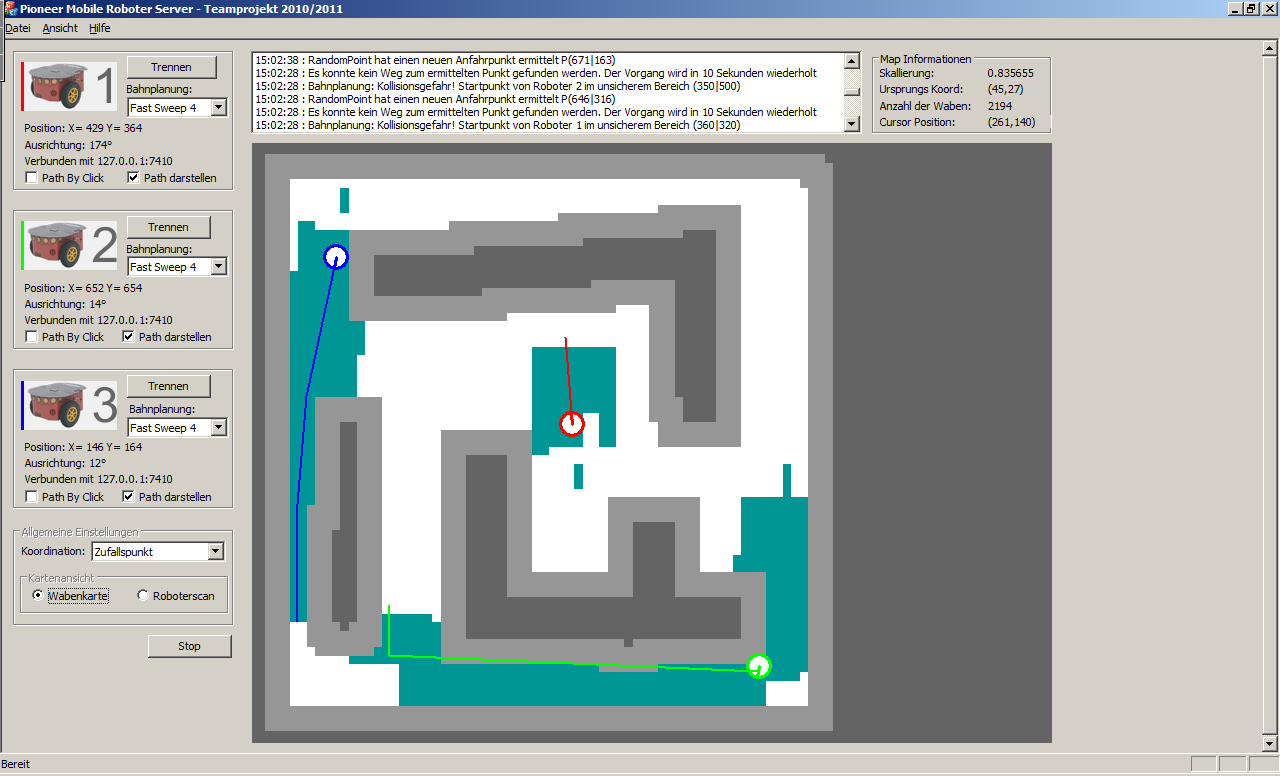
\includegraphics[width=0.5\linewidth]{bilder/avoidCollision2}
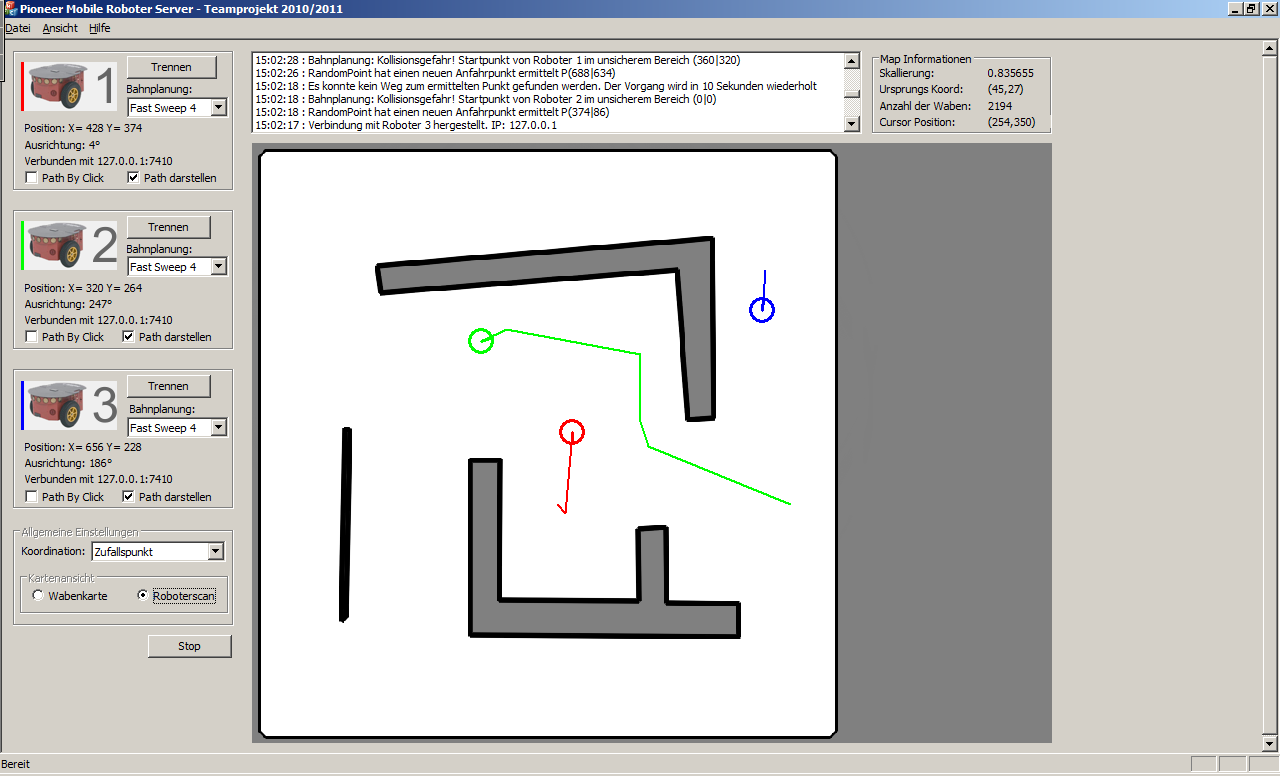
\includegraphics[width=0.5\linewidth]{bilder/avoidCollision1}
\caption{Waben- und Roboterscankarte beim Test der
  Kollisionserkennung}
\label{fig:kollisonsvermeidung}
\end{figure}
%\end{nofloat}
%\end{addmargin}
% Entsprechend arbeiten konnten, da unsere Laptops schon durch den
%ersten Roboter, sowie den Server ,,belegt'' waren. Somit konnten wir
%mit dem realen Roboter nur testen, ob die Kollision mit Wänden
%vermieden wurde. Dies klappte in der Tat ohne Probleme. 
Danach haben wir getestet, ob die Erkennung der Wände auch mit einen
Roboter im Raum vor dem Robotiklabor im Braunschweiger
Informatikzentrum funktionieren würde. Wie oben erwähnt, hatte dieser
deutlich geringeres Problempotential. Wie erwartet klappte dann auch
die Vermeidung der Wände ohne Probleme. Nur einmal wurde eine Wand
doch angefahren. \newpage Dies war darauf zurückzuführen, dass die
Positionserkennung  mit dem Sonar-Partikelfilter kurzfristig einen
Ausreißer hatte (vgl. hierzu auch den Abschnitt
\ref{sec:lokal-mit-den} ab Seite \pageref{sec:lokal-mit-den}). Somit
war aus Sicht der Kollisonsvermeidung keine Gefahr vorhanden und
brauchte somit auch nicht abgewehrt werden. Im Endeffekt ist dieser
,,Fehlschlag'' also kein Zeichen, dass die Kollisionsvermeidung nicht
funktionieren würde. \\\\
%Um nun das Verhalten der Bahnplanung und Kollisionsvermeidung bei
%mehreren Robotern zu testen, wurde auf den im Abschnitt
%\ref{serv:testclient} auf Seite \pageref{serv:testclient}
%beschriebenen Testclient zurückgegriffen, der das Verhalten des
%Clients emuliert. Wir haben insgesamt drei virtuelle Testclients mit
%dem Server verbunden und konnten somit die Kollisionsvermeidung testen.
%Bei der Bahnplanung ergab sich das Problem, dass uns nur ein Roboter
%zum Testen zur Verfügung 
%input{eva_bahnplanung}
%\input{eva_kollision}
%Client-Server Kommunikation, die Bahnplanung und Kollisionsvermei
%%% Local Variables:
%%% mode: latex
%%% TeX-master: "template"
%%% End:

\section{Evaluierung des Clients}
\subsection{Lokalisierung mit den Sonar-Partikelfilter}
\label{sec:lokal-mit-den}
Bei unseren Versuchen die Position des Roboters im Raum zu bestimmen,
stiessen wir recht früh auf Probleme: So wurde regelmäßig eine
komplett falsche Position im Raum bestimmt oder aber (gerade wenn der
Roboter sich nahe einer Wand befand) die dem Roboter gegenüberliegende
Position am anderen Ende des Raums als Position erkannt.  Nach
mehreren Versuchen stellten wir schließlich fest, dass die
Lokalisierung besonders zuverlässig war, wenn der Roboter beim Start
des Clients sich in der Mitte des Raums befand, sodass bei der
Initialisierung des Partikelfilters durch die initiale Rotation der
Abstand zu den Wänden zu beiden Seiten gleich war. Um nun der Ursache
dieses Phänomens auf die Spur zu kommen, haben wir dann unser eigenes
Visualisierungsskript geschrieben. Wir beschreiben nun zunächst die
Funktionsweise und Installation des Skriptes, bevor wir uns den
Ergebnissen zuwenden.
\input{visualisierung}

%\input{visualisierung}

%%% Local Variables:
%%% mode: latex
%%% TeX-master: "template"
%%% End:


\section{False Positives bei der Ballerkennung}
\label{sec:false-positives-bei}
Wie bereits im Abschnitt \ref{sec:balldetection} erwähnt, kann es bei
der Ballerkennung zu False Positives kommen. Diese liegen in der
Funktionsweise der Ballerkennung begründet: Nach Aufnahme des
Kamerabildes wird das Bild vom RGB- in den HSV-Farbraum umgewandelt,
der anschließend nach roten Partikeln gefiltert wird. Erreichen diese
einen gewissen Schwellwert, werden diese nach kreisförmigen Objekten
durchsucht. Anschließend wird die Wahrscheinlichkeit berechnet, ob es
sich dabei um einen Ball handelt. Wenn nun aber im Kamerabild so ein
rotes Objekt ist (z.B: Ein anderer p3dx-Roboter), wird dieses mit
hoher Wahrscheinlichkeit als ,,Ball'' erkannt. In unseren Versuchen
wurden unter anderen der Feuerlöscher des Labors, aber auch die roten
Schränke gerne als ,,Bälle'' erkannt. Dies konnten wir durch Aufbau
eines geeigneten Sichtschutzes verhindern, allerdings kam es immer
noch zu false Positives an Stellen, wo weder ein rotes Objekt, noch
sonst irgendein Objekt vorhanden war. Wir konnten schließlich durch
Rückfrage mit Tobias Breuer klären, dass dann höchstwahrscheinlich im
Licht der den Vorraum des Fahrstuhl vor dem Robotiklabor beleuchtenden
Lampen soviele Rot-Partikel vorhanden sind, dass auch da unter
Umständen false Positives auftauchen können. Aus Zeitgründen war es
uns leider nicht mehr möglich zu testen, ob das Ausschalten der Lampen
zu einer Verbesserung geführt hätte. An und für sich wäre das aber die
logische Konsequenz aus der vermuteten Ursache und auch die leichteste
Möglichkeit, diese Vermutung auf ihren Wahrheitsgehalt zu überprüfen.

%%% Local Variables:
%%% mode: latex
%%% TeX-master: "template"
%%% End:


%%% Local Variables:
%%% mode: latex
%%% TeX-master: "template"
%%% End:

%\subsection{Lokalisierung mit den Sonar-Partikelfilter}
\label{sec:lokal-mit-den}
Bei unseren Versuchen die Position des Roboters im Raum zu bestimmen,
stiessen wir recht früh auf Probleme: So wurde regelmäßig eine
komplett falsche Position im Raum bestimmt oder aber (gerade wenn der
Roboter sich nahe einer Wand befand) die dem Roboter gegenüberliegende
Position am anderen Ende des Raums als Position erkannt.  Nach
mehreren Versuchen stellten wir schließlich fest, dass die
Lokalisierung besonders zuverlässig war, wenn der Roboter beim Start
des Clients sich in der Mitte des Raums befand, sodass bei der
Initialisierung des Partikelfilters durch die initiale Rotation der
Abstand zu den Wänden zu beiden Seiten gleich war. Um nun der Ursache
dieses Phänomens auf die Spur zu kommen, haben wir dann unser eigenes
Visualisierungsskript geschrieben. Wir beschreiben nun zunächst die
Funktionsweise und Installation des Skriptes, bevor wir uns den
Ergebnissen zuwenden.
\section{Visualisierung der Partikelmengen des Partikelfilters}
Da die im Partikelfilter integrierte Visualisierung der Partikelmenge
nicht immer funktionierte und es auch keine direkte SPeichermöglichkeit der
 Bilder gab, haben wir den Partikelfilter, so erweitert, dass die
Partikelmenge in eine Datei geschrieben werden kann (
\ref{sec:sonarparticlefilter}) und passend dazu ein Skript (in Python unter
 Benutzung von pygame geschrieben), welches die Partikel anhand der Daten
 aus einer Partikelmengendatei über ein Bild legt. Dieses ist im Ordner
 Visualisierung im SVN-Repository unter dem Namen visualize.py zu finden.

 \subsection{HOWTO: Installieren der Abhängigkeiten des
Visualisierungsskriptes und Benutzung dessen}
 \begin{itemize}
	 \item Python 3.2 herunterladen und installieren\footnote{http://python.org/ftp/python/3.2.2/python-3.2.2.msi}
	 \item pygame 1.9.2a0 für Python 3.2 installieren \footnote{http://pygame.org/ftp/pygame-1.9.2a0.win32-py3.2.msi}
	 \item Python 3.2 zum PATH hinzufügen
	 \item cmd/Eingabeaufforderung öffnen
	 \item In den Ordner Visualisierung des Repositories wechseln
	 \item Das Visualisierungsskript kann nun folgendermaßen benutzt werden:\\
	 		\lstinline|python visualize.py (Dateiname des Bildes) (Dateiname der Partikelmengendatei)| \\
 			z.b. \lstinline|python visualize.py OccuMap.bmp visual.log|
	 \item Das Ausgabebild hat dann den Namen V\_(Dateiname der Partikelmengendatei)\_(Dateiname des Bildes)
\end{itemize}

%\section{Visualisierung der Partikelmengen des Partikelfilters}
Da die im Partikelfilter integrierte Visualisierung der Partikelmenge
nicht immer funktionierte und es auch keine direkte SPeichermöglichkeit der
 Bilder gab, haben wir den Partikelfilter, so erweitert, dass die
Partikelmenge in eine Datei geschrieben werden kann (
\ref{sec:sonarparticlefilter}) und passend dazu ein Skript (in Python unter
 Benutzung von pygame geschrieben), welches die Partikel anhand der Daten
 aus einer Partikelmengendatei über ein Bild legt. Dieses ist im Ordner
 Visualisierung im SVN-Repository unter dem Namen visualize.py zu finden.

 \subsection{HOWTO: Installieren der Abhängigkeiten des
Visualisierungsskriptes und Benutzung dessen}
 \begin{itemize}
	 \item Python 3.2 herunterladen und installieren\footnote{http://python.org/ftp/python/3.2.2/python-3.2.2.msi}
	 \item pygame 1.9.2a0 für Python 3.2 installieren \footnote{http://pygame.org/ftp/pygame-1.9.2a0.win32-py3.2.msi}
	 \item Python 3.2 zum PATH hinzufügen
	 \item cmd/Eingabeaufforderung öffnen
	 \item In den Ordner Visualisierung des Repositories wechseln
	 \item Das Visualisierungsskript kann nun folgendermaßen benutzt werden:\\
	 		\lstinline|python visualize.py (Dateiname des Bildes) (Dateiname der Partikelmengendatei)| \\
 			z.b. \lstinline|python visualize.py OccuMap.bmp visual.log|
	 \item Das Ausgabebild hat dann den Namen V\_(Dateiname der Partikelmengendatei)\_(Dateiname des Bildes)
\end{itemize}

%%% Local Variables:
%%% mode: latex
%%% TeX-master: "template"
%%% End:

%\section{Visualisierung der Partikelmengen des Partikelfilters}
Da die im Partikelfilter integrierte Visualisierung der Partikelmenge
nicht immer funktionierte und es auch keine direkte SPeichermöglichkeit der
 Bilder gab, haben wir den Partikelfilter, so erweitert, dass die
Partikelmenge in eine Datei geschrieben werden kann (
\ref{sec:sonarparticlefilter}) und passend dazu ein Skript (in Python unter
 Benutzung von pygame geschrieben), welches die Partikel anhand der Daten
 aus einer Partikelmengendatei über ein Bild legt. Dieses ist im Ordner
 Visualisierung im SVN-Repository unter dem Namen visualize.py zu finden.

 \subsection{HOWTO: Installieren der Abhängigkeiten des
Visualisierungsskriptes und Benutzung dessen}
 \begin{itemize}
	 \item Python 3.2 herunterladen und installieren\footnote{http://python.org/ftp/python/3.2.2/python-3.2.2.msi}
	 \item pygame 1.9.2a0 für Python 3.2 installieren \footnote{http://pygame.org/ftp/pygame-1.9.2a0.win32-py3.2.msi}
	 \item Python 3.2 zum PATH hinzufügen
	 \item cmd/Eingabeaufforderung öffnen
	 \item In den Ordner Visualisierung des Repositories wechseln
	 \item Das Visualisierungsskript kann nun folgendermaßen benutzt werden:\\
	 		\lstinline|python visualize.py (Dateiname des Bildes) (Dateiname der Partikelmengendatei)| \\
 			z.b. \lstinline|python visualize.py OccuMap.bmp visual.log|
	 \item Das Ausgabebild hat dann den Namen V\_(Dateiname der Partikelmengendatei)\_(Dateiname des Bildes)
\end{itemize}


%%% Local Variables:
%%% mode: latex
%%% TeX-master: "template"
%%% End:
%Beschreibung einiger Versuche (sowohl erfolgreich), 
                  %als auch der fails (Lokalisierung nur in Mitte des 
                  %Raumes zuverlässig, Balldetection gibt 
                  %falsePositives wenn weißes Licht zuviele rote 
                  %Partikel enthält) 

\chapter{Zusammenfassung}
\label{cha:zusammenfassung}
Unsere Aufgabenstellung eine koordinierte Ballsuche 
zu implementieren, ist uns im Wesentlichen gelungen:\\
Ein zentraler Server nimmt die Bahnplanung vor und ist in der Lage die
Bahnplanung für bis zu drei Clients vorzunehmen. Diese Bahn wird von
der Clientsoftware ohne größere Probleme abgefahren. Mit der Hilfe der
uns zur Verfügung stehenden Ballerkennung von Tobias Breuer und des
auf einen früheren Teamprojekt aufbauenden Sonar-Partikelfilters war
es möglich, ohne größeres Hintergrundwissen, den Client so zu
entwickeln, dass er nicht nur seine eigene Position im Raum, sondern
auch enventuell dort vorhandene Bälle bestimmen kann. \\\\
Zwar erwies sich der Partikelfilter in bestimmten Situationen als nur
bedingt zuverlässig, diese Problematik lässt sich aber durch ein
geschickte Wahl der Initialisierungsposition umgehen. Theoretisch wäre
es auch denkbar, die Roboter zusätzlich zum eingebauten Sonar mit
einen Laserscanner auszustatten, dieser sollte vom Ansatz her deutlich
zuverlässigere Ergebnisse liefern. Eine Implementierung dieses
Ansatzes lag allerdings nicht im Fokus unseres Projektes. \\\\
Grundsätzlich kann also das Projekt als Erfolg betrachtet werde.n
%%% Local Variables:
%%% mode: latex
%%% TeX-master: "template"
%%% End:
 % Zusammenfassung halt :) 
 
 
% \begin{appendix} 
% dazu anhang mit installationsanleitung und ggf. weiteren Kram. 
%\section{Integration bestehender Projekte in ein neues Buildsystem für den
Client}
\label{cha:integr-best-proj}
\subsection{Warum ein neues Buildsystem?}
Die Ballerkennung und der Sonarpartikelfilter hängen von vielen
Altprojekten
ab. Das Beispiel für die Steuerung der Pioneer 3-DX hing zudem von der ARIA
Bibliothek\footnote{http://robots.mobilerobots.com/wiki/ARIA} ab. Bei den
Altprojekten fanden sich auch zum Teil fest kodierte Pfade. Da auch die
Konvertierung der Solutions in das VS 2010 Format meistens fehlschlug und
auch
ARIA nicht mit der mitgelieferten Solution unter VS 2010 gebaut werden
konnte,
haben wir uns für den Client für den Einsatz eines neuen Buildsystems
entschlossen. Aufgrund der Einfacheit der Beschreibung der Buildvorgänge
für
die einzelnen zu integrierenden Projekte und dem Hinzufügen neuer
Unterprojekte, sowie der Möglichkeit, von einem konkreten Buildsystem
abhängig
zu sein sowie existierender Erfahrungen mit dem System, fiel die Wahl auf
CMake\footnote{http://www.cmake.org/}. Bei CMake handelt es sich um ein
open-source Metabuildsystem. Es erzeugt Build-Vorschriften für andere
Buildsysteme (u.a. GNU make, nmake, msbuild). Somit wäre es bei Bedarf auch
Möglich gewesen, auf eine andere Visual Studio Version umzusteigen ohne
die Solutions zu konvertieren oder neu zu erstellen.

\subsection{Integration der Projekte}
Zuerst wurde eine passende Ordnerstrukur angelegt: include für
Header-Dateien,
src für die cpp-Dateien der einzelnen Projekt, bin für eventuell zum Linken
 benötigte
Kompillate, deren Quellen nicht in den Build-Prozess integrierbar waren und
build als Zielordner für erzeugte Buildfiles.

Als nächstes wurde für das Projekt im Ordner des Clients eine
CMakeLists.txt-Datei angelegt:

\begin{lstlisting}[language={},captionpos=b,caption={CMakeLists.txt für das Buildsystem des Clients}]
cmake_minimum_required (VERSION 2.6)
project (TP_WS_2010)

include_directories (include)
include_directories (include/ControlExample)
include_directories (include/erob/)
include_directories (include/Balldetection)
include_directories (include/p3dxSteuerung)
include_directories (include/StochasticLib)
include_directories (include/PioneerMRClient)
include_directories (include/Aria)
include_directories (include/OccupancyGridMap)
include_directories (include/irpVideo/DirectShow)
link_directories (${TP_WS_2010_BINARY_DIR})
link_directories (${TP_WS_2010_SOURCE_DIR}/lib/)
add_subdirectory (src)
\end{lstlisting}

Diese definiert den Namen des Projektes (wichtig
für Referenzen auf z.b. das Stammverzeichnis des Projektes oder das
Buildverzeichnis, da die entprechenden Variablennamen mit dem Projektnamen
+ \_
als Präfix versehen werden. Zudem wurden die include-Verzeichnisse und zum
Linken relevante Verzeichnisse festgelegt. Danach wurde das src-Verzeichnis
 als
Projektunterordner hinzugefügt. Dadurch werden die Anweisungen in der
CMakeLists.txt des Unterordners auch ausgeführt. Dies ermöglicht es, für
die
einzelnen Unterprojekte jeweils eine eigene kleine CMakeLists.txt zu
verwenden.

Die CMakeLists.txt bindet nun alle Sourceordner der Unterprojekte ein:

\begin{lstlisting}[language={},captionpos=b,caption={CMakeLists.txt für den Sourceordner}]
%\begin{lstlisting}
cmake_minimum_required (VERSION 2.6)

add_subdirectory (irpUtils)
add_subdirectory (irpMath)
add_subdirectory (irpImage)
add_subdirectory (irpVideo)
add_subdirectory (irpFeatureExtraction)
add_subdirectory (alglib)
add_subdirectory (DistanceMap)
add_subdirectory (irpCamera)
add_subdirectory (irpV3d)
add_subdirectory (StochasticLib)
add_subdirectory (Visualization)
add_subdirectory (CamCalib)
add_subdirectory (Balldetection)
add_subdirectory (mathtest)
add_subdirectory (SonarParticleFilter)
add_subdirectory (PioneerMRClient)
add_subdirectory (OccupancyGridMap)
add_subdirectory (Balldetection_Test)
add_subdirectory (Aria)
add_subdirectory (p3dxSteuerung)
add_subdirectory (p3dxSteuerung_threaded)
add_subdirectory (calibrate)
#add_subdirectory (ControlExample)
add_subdirectory (utils)
add_subdirectory (kinect)
add_subdirectory (networkTest)
\end{lstlisting}

Bei den Unterprojekten gibt es zwei Arten: Bibliotheken und Anwendungen.

Die CMakeList.txt einer Bibliothek sieht wie folgt aus:
\begin{lstlisting}[language={},captionpos=b,caption={CMakeLists.txt einer Bibliothek am
    Beispiel irpCamera}]
%\begin{lstlisting}
cmake_minimum_required (VERSION 2.6)

file(GLOB src "*.cpp")
file(GLOB includes "../../include/irpCamera/*.h")

add_library (irpCamera ${src} ${includes})
\end{lstlisting}

Die CMakeList.txt einer Anwendung sieht so aus:
\begin{lstlisting}[language={},captionpos=b,caption={CMakeLists.txt des Clients}]
cmake_minimum_required (VERSION 2.6)

file(GLOB src "*.cpp")
file(GLOB includes "../../include/p3dxSteuerung/*.h")
add_executable (p3dxSteuerung_threaded ${src} ${includes})
target_link_libraries (p3dxSteuerung_threaded irpUtils MINPACK fftw rfftw
DirectShow irpFeatureExtraction irpMath  alglib irpImage irpCamera irpVideo
 irpV3d glew CamCalib Visualization StochasticLib OccupancyGridMap
SonarParticleFilter ws2_32 winmm advapi32 Aria DistanceMap Balldetection)

\end{lstlisting}

Zuerst werden alle cpp-Dateien zur Variablen src hinzugfügt, danach die
Includes zur Variablen include. Je nachdem, ob es sich um eine Bibliothek
oder
Anwendung handelt, wird diese mit add\_library(name dateien) oder
add\_executable(name dateien) hinzugefügt. Die Include-Dateien müssen dabei
aber eigentlich nicht explizit hinzugefügt werden, dies geschieht nur,
damit
sie auch in einer VS Solution in der Dateiliste auftauchen. Bei Anwendungen
können nun mit target\_link\_libraries(exename libraries) noch die zu
linkenden
Bibliotheken angegeben werden.

Es gab ein paar Probleme bei der Integration: zum einen mussten zuerst die
Abhängigkeiten zwischen den Unterprojekten ermittelt werden, dies geschah
mit
Hilfe der originalen VS Solutions sowie durch Ausprobieren. Zum anderen gab
 es
manchmal Dateien, die zwar in den Quellen lagen, jedoch in nicht in den
Solutions auftauchten. Diese konnten den Buildprozess stören und mussten
daher
entfernt werden TODO: Beispiel raussuchen, wenn noch überhaupt möglich.
Außerdem waren an ein paar Stellen kleinere Änderungen am Quellcode nötig,
um
ihn mit MSVC 2010 oder der Struktur unseres include-Ordners kompatibel zu
machen.

\subsection{Hinzufügen eines neuen Unterprojektes}
\label{sec:hinz-eines-neuen-unterprojektes}
Das Hinzufügen eines neuen Unterprojektes ist relativ einfach.
Zuerst wird ein Unterverzeichnis für das Projekt im include-Ordner und
eines im
src-Ordner angelegt. Dann kopiert man die includes in den neuen Unterordner
 im
include-Ordner. Dabei ist darauf zu achten, dass die Pfade in
\#include-Direktiven relative zum include-Ordner sein sollten. Danach
kopiert
man die cpp-Dateien in den neuen Unterordner im src-Verzeichnis.

Danach erstellt man in diesem Ordner eine CMakeLists.txt ähnlich wie oben,
jenachdem ob ex sich um eine Anwendung oder Bibliothek handelt. Man fügt
zuerst
die cpp-Dateien und Includes hinzu, fügt dann mit add\_library oder
add\_executable Buildtargets hinzu und gibt eventuell noch zu linkende
Bibliotheken bei Anwendungen an mit target\_link\_libraries.

%%% Local Variables: 
%%% mode: latex
%%% TeX-master: "template"
%%% End: 
 
%\end{appendix} 
 
%literatur? Vielleicht die quelle des bahnplanungsalgorithmuses? 
%\begin{thebibliography}{99} 
%        \addcontentsline{toc}{chapter}{Bibliography} 
%        \bibitem[HORST06]{horst}\textsc{Horstmann, Werner}: 
%        \textsl{Das Fressverhalten der gemeinen Steinlaus bei Gegenlicht}. 
%        Springer, Berlin, March 2006. 
% 
% 
%\end{thebibliography} 
 
 
 
\end{document} 
 
 
%%% Local Variables:  
%%% mode: latex 
%%% TeX-master: t 
%%% End:  
